\appendix
\counterwithin{table}{section}
\counterwithin{figure}{section}

\section{Sensitivity and robustness}\label{app:sens}

\subsection{Compound rates and seasons}

Table~\ref{tab:rates} gives the 2026 rates behind Figure~\ref{fig:circuit}A.
Table~\ref{tab:seasons} repeats the race model for each season with weekend labels in place of physical compounds.
The circuit-slope standard deviation ranges from \CircuitSDSeasonTwentyFive{} to \CircuitSDSeasonTwentySix\spl, and the within-event compound trend has the textbook sign in 2022, 2023 and 2025 and is indistinguishable from zero in 2024 and 2026.

\begin{table}[t]
\centering\small
\begin{tabular}{@{}lrrrr@{}}
\toprule
Compound & Runs & Laps & Rate (s/lap) & 95\% interval \\
\midrule
C1 & 55 & 801 & 0.0410 & [0.0079, 0.0742] \\
C2 & 191 & 2{,}836 & 0.0373 & [0.0081, 0.0665] \\
C3 & 242 & 3{,}316 & 0.0544 & [0.0258, 0.0830] \\
C4 & 223 & 2{,}943 & 0.0633 & [0.0346, 0.0921] \\
C5 & 109 & 1{,}143 & 0.0385 & [0.0090, 0.0680] \\
\midrule
2026 circuit-slope SD (13 circuits, one race each) &  &  & 0.0498 & [0.0354, 0.0810] \\
SD of the five compound rates &  &  & 0.0114 &  \\
Within-event trend per step softer &  &  & \ensuremath{-}0.0010 & [\ensuremath{-}0.0047, \ensuremath{+}0.0028] \\
\bottomrule
\end{tabular}

\caption{Race degradation rate per compound in 2026 (seconds lost per lap of tyre age) from the mixed model of Eq.~\eqref{eq:race}, with 95\% Wald intervals. The circuit-slope standard deviation has a 95\% profile-likelihood interval. The last row is the within-event trend per step from a harder to a softer compound, estimated with one fixed slope per event (negative means softer compounds degrade more slowly within the same race).}
\label{tab:rates}
\end{table}

\begin{table}[t]
\centering\small
\begin{tabular}{@{}lrrl@{}}
\toprule
Season & Circuits & Circuit-slope SD (s/lap) & Within-event trend per step softer \\
\midrule
2022 & 18 & 0.0430 & \ensuremath{+}0.0109 [0.0040, 0.0179] \\
2023 & 16 & 0.0309 & \ensuremath{+}0.0024 [\ensuremath{-}0.0046, 0.0095] \\
2024 & 18 & 0.0258 & \ensuremath{+}0.0001 [\ensuremath{-}0.0064, 0.0065] \\
2025 & 17 & 0.0235 & \ensuremath{+}0.0048 [\ensuremath{-}0.0031, 0.0127] \\
2026 & 13 & 0.0439 & \ensuremath{-}0.0112 [\ensuremath{-}0.0177, \ensuremath{-}0.0048] \\
\bottomrule
\end{tabular}

\caption{Race model by season with hard, medium and soft labels in place of the physical compounds of Table~\ref{tab:rates}, so the 2026 row differs slightly from it (circuit-slope SD and within-event trend). The within-event trend is the change in degradation rate (s/lap) per step from a harder to a softer label with one slope per event, with a 95\% Wald interval; positive is the textbook sign.}
\label{tab:seasons}
\end{table}

\subsection{Inference under alternative error structures}\label{app:inference}

Table~\ref{tab:inference} gives the width of the 95\% interval for each 2026 compound rate under six ways of counting independent information.
Treating laps as independent produces the narrowest intervals; circuit slopes, run intercepts and run slopes each widen them and reduce the residual autocorrelation within runs.
The last two rows use fixed-effects regressions with cluster-robust errors, which allow any correlation within a run or within an event, including the correlation that demeaning induces.
Clustering by event, with a $t$ reference on 12 degrees of freedom, gives intervals narrower than ours for every compound, so the correlation we do not model does not make our intervals too narrow.

\begin{table}[t]
\centering\footnotesize\setlength{\tabcolsep}{4pt}
\begin{tabular}{@{}lrrrrrr@{}}
\toprule
Inference & C1 & C2 & C3 & C4 & C5 & Lag-1 autocorr. \\
\midrule
Laps independent, no circuit slope & 0.025 & 0.011 & 0.007 & 0.008 & 0.011 & -- \\
Laps independent, circuit slope & 0.053 & 0.042 & 0.040 & 0.041 & 0.042 & 0.36 \\
Circuit slope, run intercepts & 0.069 & 0.048 & 0.046 & 0.047 & 0.048 & 0.26 \\
Circuit slope, run intercepts and slopes (ours) & 0.082 & 0.055 & 0.052 & 0.053 & 0.057 & 0.23 \\
Fixed effects, errors clustered by run & 0.023 & 0.021 & 0.014 & 0.016 & 0.031 & -- \\
Fixed effects, errors clustered by event, $t_{12}$ & 0.024 & 0.056 & 0.032 & 0.044 & 0.053 & -- \\
\bottomrule
\end{tabular}

\caption{Width of the 95\% interval (s/lap) for each 2026 compound rate under alternative inference. The first four rows are mixed models of Eq.~\eqref{eq:race} with progressively more random effects; ``ours'' is the specification used throughout. The last two rows are regressions with driver-in-event fixed effects and cluster-robust standard errors; they omit the circuit and run terms, so their point estimates differ from the mixed models (for C4 and C5 by about half) and only their widths are compared here. The last column is the residual lag-1 autocorrelation within runs, where defined.}
\label{tab:inference}
\end{table}

\subsection{Why a cross-sectional race estimator fails}\label{app:xs}

A cross-sectional alternative to Eq.~\eqref{eq:race} regresses lap time on tyre age within each event, lap and compound, with no run terms.
It compares cars of different tyre age on the same lap, but who is on older tyres depends on pit timing, which depends on strategy and car pace, so tyre age is correlated with unmodelled pace.
The estimator returns negative soft slopes, and for the race-only trend across compounds it gives \ReconCrossSectionalAll\spl{} per step over all seasons.
Run intercepts in Eq.~\eqref{eq:race} absorb each run's pace level, so the slope is no longer driven by who has stopped.
We therefore do not interpret the cross-sectional estimate.

The sign of the race-only trend across compounds depends on how the slope is identified.
Within-run contrasts, which compare a car with itself, give \ReconWithinRunAll\spl{} per step softer [\ReconWithinRunAllLo, \ReconWithinRunAllHi] over all seasons, and the race contrasts of the fixed-effects design in Table~\ref{tab:racepractice} are about \DidTWFESoftHardRaceContrast\spl{} between each pair of compounds.
A field-demeaned slope without run terms, which compares cars with each other on the same lap, gives \ReconFieldDemeanedAll\spl{} on the same groups, the sign error that run terms remove.
The two kinds of design answer different questions, and the fixed-effects race contrasts are means over only the events that have practice sessions.

\subsection{Exploratory specifications for the management test}

The analysis of race against practice has many analyst choices \citep{gelman2014crisis}.
As an exploratory check, we re-ran the trend test of Section~\ref{sec:gap} over \MultiverseSpecs{} alternative specifications that vary the assumed fuel burn (1.4, 1.7 and 2.0\,kg per lap) and fuel effect (0.025, 0.033 and 0.040\,s/kg), the tyre-age window, run length, the minimum number of runs per group, whether sprints count as practice, the season set and the race estimator.
\MultiverseNegative{} of \MultiverseSpecs{} trends are negative and \MultiverseExcludesZero{} have bootstrap intervals that exclude zero.
Because the same fuel constant is added to every slope, it leaves the trend and the gap unchanged and moves only levels and ratios.

\subsection{Practice design choices}

Practice runs are cleaned by choices that could affect the forecast of Section~\ref{sec:transfer}.
Out of season, keeping runs bridged across short gaps changes MAE by \KeepRunsDiff\spl{} relative to the main frame [\KeepRunsDiffLo, \KeepRunsDiffHi] over \KeepRunsCommonCells{} groups (negative means the variant is better), and in 2026 trimming the warm-up lap changes it by \WarmupDiff\spl{} [\WarmupDiffLo, \WarmupDiffHi] (sign-flip $p=\WarmupSignFlipP$).
The main frame has \PracticeLapsShipped{} laps against \PracticeLapsLegacy{} for the earlier design.
The choices make small differences that we do not treat as evidence for any one design.

\subsection{Naive and fuel-corrected estimators}\label{app:ablation}

Figure~\ref{fig:sign} compares three estimators of the 2026 race rates on the same laps: the naive regression, the fuel-corrected regression within runs and the adjusted model of Eq.~\eqref{eq:race}.
The naive regression has the wrong sign for C1, C3 and C5 (\NaiveCOne, \NaiveCThree{} and \NaiveCFive\spl) and \NaiveCTwo\spl{} for C2, consistent with tyre age being confounded with fuel burn, pit-stop timing and traffic.
The fuel-corrected regression is much closer to the adjusted model, differing from it by \AblGapCThree\spl{} at C3 and \AblGapCOne\spl{} at C1.
The remaining difference may reflect track evolution and traffic, which the fuel-corrected regression does not control.

\begin{figure}[t]
\centering
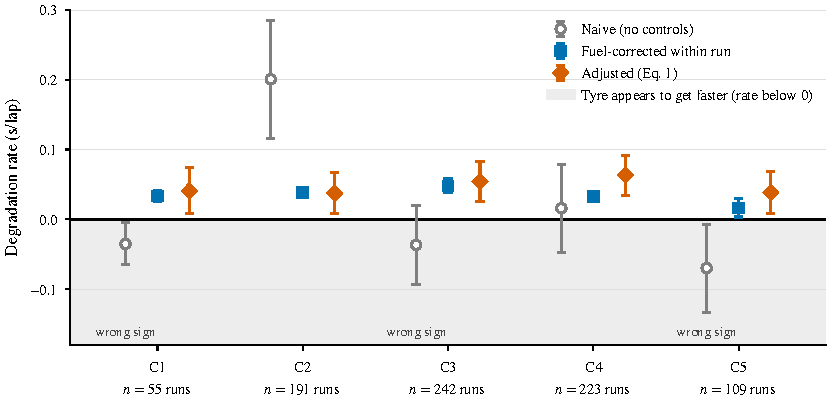
\includegraphics[width=\linewidth]{figures/fig_sign_error.pdf}
\caption{Race degradation rate per compound in 2026 under three estimators applied to the same laps: naive (open circle), fuel-corrected within runs (filled square) and adjusted, Eq.~\eqref{eq:race} (filled diamond). Markers are estimates and bars 95\% intervals (run-clustered for the naive and fuel-corrected estimators, Wald for the mixed model). Rates below zero, marked by the shaded band, mean that the tyre appears to get faster with age; $n$ is the number of runs.}
\label{fig:sign}
\end{figure}

\subsection{Race versus practice under every design}

Table~\ref{tab:racepractice} lists the gap for each compound under the primary used-set design, the other designs, the placebo and the compound contrasts behind the management test.

\begin{table}[t]
\centering\footnotesize\setlength{\tabcolsep}{3pt}
\begin{tabular}{@{}lrrrllr@{}}
\toprule
 & $n$ & Race & Practice & Difference [95\% CI] & Ratio [95\% CI] & $p$ (Holm) \\
\midrule
\multicolumn{7}{@{}l}{\textit{Used sets in both contexts (primary): 105 groups, 67 event-seasons}} \\
Hard & 23 & 0.051 & 0.107 & \ensuremath{-}0.056 [\ensuremath{-}0.116, 0.005] & 0.48 [0.20, 1.10] &  \\
Medium & 47 & 0.063 & 0.101 & \ensuremath{-}0.038 [\ensuremath{-}0.084, 0.009] & 0.63 [0.37, 1.15] &  \\
Soft & 35 & 0.076 & 0.156 & \ensuremath{-}0.080 [\ensuremath{-}0.142, \ensuremath{-}0.026] & 0.49 [0.22, 0.79] &  \\
Medium + soft & 82 & 0.071 & 0.127 & \ensuremath{-}0.056 [\ensuremath{-}0.096, \ensuremath{-}0.019] & 0.56 [0.36, 0.81] &  \\
All & 105 & 0.067 & 0.125 & \ensuremath{-}0.059 [\ensuremath{-}0.093, \ensuremath{-}0.024] & 0.53 [0.36, 0.75] &  \\
\midrule
\multicolumn{7}{@{}l}{\textit{Other designs, medium + soft}} \\
Start-age matched & 76 & 0.060 & 0.159 & \ensuremath{-}0.099 [\ensuremath{-}0.154, \ensuremath{-}0.050] & 0.38 [0.12, 0.62] &  \\
Used sets, start-age matched & 48 & 0.090 & 0.147 & \ensuremath{-}0.058 [\ensuremath{-}0.106, \ensuremath{-}0.012] & 0.61 [0.39, 0.90] &  \\
No matching & 118 & 0.059 & 0.139 & \ensuremath{-}0.079 [\ensuremath{-}0.118, \ensuremath{-}0.041] & 0.43 [0.29, 0.61] &  \\
\midrule
\multicolumn{7}{@{}l}{\textit{Placebo: practice 2 (first column) against practice 1 and 3, used sets}} \\
Medium + soft & 63 & 0.150 & 0.156 & \ensuremath{-}0.006 [\ensuremath{-}0.053, 0.037] & 0.96 [0.72, 1.32] &  \\
All & 76 & 0.148 & 0.152 & \ensuremath{-}0.003 [\ensuremath{-}0.049, 0.038] & 0.98 [0.75, 1.34] &  \\
Gap minus placebo gap &  &  &  & \ensuremath{-}0.050 [\ensuremath{-}0.106, 0.007] &  &  \\
\midrule
\multicolumn{7}{@{}l}{\textit{Compound slope contrast per context, and difference in differences, per event}} \\
Soft $-$ hard & 21 & \ensuremath{+}0.018 & \ensuremath{+}0.089 & \ensuremath{-}0.071 [\ensuremath{-}0.134, \ensuremath{-}0.013] &  & 0.028 (0.085) \\
Soft $-$ medium & 32 & \ensuremath{+}0.018 & \ensuremath{+}0.017 & \ensuremath{-}0.006 [\ensuremath{-}0.048, 0.035] &  & 0.807 (0.807) \\
Medium $-$ hard & 31 & \ensuremath{+}0.018 & \ensuremath{+}0.064 & \ensuremath{-}0.040 [\ensuremath{-}0.085, 0.005] &  & 0.091 (0.182) \\
\bottomrule
\end{tabular}

\caption{Race and practice degradation. Italic rows are panel headings. The primary design keeps used sets in both settings; its panel lists each compound, medium and soft together (\NMatchedCellsMS{} groups, the headline in the text) and all compounds (\NMatchedCellsAll{} groups). In the first three panels $n$ is the number of race--compound groups; Race and Practice are pooled slopes (s/lap), the difference is race minus practice and the ratio is race over practice, with 95\% percentile cluster-bootstrap intervals over event-seasons. In the placebo panel the first slope column is FP2 and the second is FP1 and FP3 together. The row ``Gap minus placebo gap'' is for medium and soft, with a joint-bootstrap interval. In the last panel $n$ is the number of events, the two slope columns are the mean race and practice contrasts between the named compounds, the difference is the mean difference in differences with its 95\% bootstrap interval, and the last column is the two-sided sign-flip permutation $p$-value with its Holm-adjusted value in parentheses.}
\label{tab:racepractice}
\end{table}

\section{Checks on the race estimator}\label{app:checks}

\subsection{Exact and approximate demeaning}\label{app:exact}

Eq.~\eqref{eq:race} demeans every fixed-effect column within the (event, lap) group: the compound indicators $\tilde D_{c}$, with one compound as the reference, and their products with raw tyre age, $\widetilde{(D_c a)}$.
Our first analysis instead used the raw indicators for the offsets and the indicator times tyre age demeaned over all cars, $D_c\,\tilde a$, for the slopes.
The two coincide when every car on a lap uses the same compound, which is rare in a race.
When compounds are mixed, $D_c\,\tilde a$ measures a car's tyre age against cars on other compounds, so it carries part of the other compounds' offsets and slopes, and the error falls hardest on compounds that run at few races or alongside many others.
Table~\ref{tab:exact} fits both constructions to the same laps with the same random effects and the same REML engine.
In 2026 the approximate construction roughly doubles the C1 rate and halves the C5 rate, which reverses the apparent order of the compounds; pooled over 2022--26 it compresses the five rates towards each other, cutting their standard deviation from \PooledCompoundSD{} to \ApproxPoolCompoundSD\spl, while the circuit component moves less (\PersistSD{} against \ApproxPoolCircuitSD\spl).
In the recovery study below, the approximate construction is biased for the compound at the edge of the allocation (C1 by about 0.013\spl) even when stops are random, and the exact one is not.

\begin{table}[t]
\centering\footnotesize\setlength{\tabcolsep}{4pt}
\begin{tabular}{@{}lrrrrrrr@{}}
\toprule
Fit & C1 & C2 & C3 & C4 & C5 & Compound SD & Circuit SD \\
\midrule
2026, exact & 0.041 & 0.037 & 0.054 & 0.063 & 0.039 & 0.0114 & 0.0498 \\
2026, approximate & 0.082 & 0.053 & 0.050 & 0.042 & 0.022 & 0.0219 & 0.0437 \\
2022--26 pooled, exact & 0.044 & 0.043 & 0.060 & 0.066 & 0.073 & 0.0134 & 0.0278 \\
2022--26 pooled, approximate & 0.056 & 0.047 & 0.058 & 0.059 & 0.053 & 0.0047 & 0.0247 \\
\bottomrule
\end{tabular}

\caption{Race degradation rate per compound (s/lap) under the exact demeaning of Eq.~\eqref{eq:race} and the approximate construction $D_c\,\tilde a$, on the same laps with the same random effects. Compound SD is the standard deviation of the five rates; circuit SD is the circuit-slope standard deviation (2026) or its persistent component (pooled).}
\label{tab:exact}
\end{table}

\subsection{Recovery of known rates}\label{app:recovery}

Each replicate simulates the 13 races of 2026 with their actual compound nominations, 20 cars and 55 laps.
Lap time is the sum of car pace, a fuel effect, track evolution that differs by race, a weather shock shared by the field, a compound offset, a tyre-age slope made of the compound rate plus circuit and run deviations, a run intercept and serially correlated noise; the variance components are close to the fitted 2026 values, and the planted compound rates span 0.02 to 0.08\spl.
There are no safety cars, retirements or traffic, which favours every estimator.
Each car makes one or two stops.
Stops fall at random laps (random), earlier and more often for slower cars (pace), or when the lap time a run has lost since its stop crosses a threshold, so that runs that degrade fast end early (wear).
All three scenarios share every random draw except the stop laps, and each has \RecReps{} replicates.

Table~\ref{tab:recovery} reports the mean bias over compounds, the mean absolute bias and the coverage of nominal 95\% intervals.
The naive regression is biased low by 0.06 to 0.08\spl{} in every scenario.
The fuel-corrected regression is biased low by \RecFuelExoBiasAbs\spl{} even with the right fuel constant, because track evolution is confounded with tyre age within a run.
The cross-sectional and field-demeaned regressions, which compare cars on the same lap without run terms, are unbiased when stops are random but have bias \RecCrossPaceBias\spl{} when slower cars stop earlier, the selection that run terms absorb.
Eq.~\eqref{eq:race} has mean absolute bias below 0.002\spl{} in both of those scenarios, with coverage \RecExactExoCov{} and \RecExactPaceCov, a little below the nominal level.
When stops are triggered by wear the identifying assumption fails, and Eq.~\eqref{eq:race} understates the rates by \RecExactWearBiasAbs\spl{} with coverage \RecExactWearCov; adding run means (Section~\ref{app:mundlak}) reduces this only slightly.
The circuit-slope standard deviation, planted at \RecTrueCircuitSD\spl, is recovered with bias \RecExactExoCircBias{} and \RecExactPaceCircBias\spl, and \RecExactWearCircBias\spl{} under wear-triggered stops.
The expectations for the first estimators were written before the first run; those for the corrected estimator were added after the correction, and the coverage band we set for it (0.925 to 0.975) is narrowly missed.

\begin{table}[t]
\centering\scriptsize\setlength{\tabcolsep}{3pt}
\begin{tabular}{@{}lrrrrrrrrr@{}}
\toprule
\multicolumn{1}{l}{} & \multicolumn{3}{c}{Random stops} & \multicolumn{3}{c}{Stops by pace} & \multicolumn{3}{c}{Stops by wear} \\
\cmidrule(lr){2-4}\cmidrule(lr){5-7}\cmidrule(l){8-10}
Estimator & Bias & $|$Bias$|$ & Cov. & Bias & $|$Bias$|$ & Cov. & Bias & $|$Bias$|$ & Cov. \\
\midrule
Naive & \ensuremath{-}0.062 & 0.062 & 0.05 & \ensuremath{-}0.077 & 0.077 & 0.02 & \ensuremath{-}0.070 & 0.070 & 0.03 \\
Fuel-corrected within run & \ensuremath{-}0.012 & 0.012 & 0.42 & \ensuremath{-}0.012 & 0.012 & 0.43 & \ensuremath{-}0.029 & 0.029 & 0.22 \\
Cross-sectional, no run terms & \ensuremath{+}0.000 & 0.000 & 0.79 & \ensuremath{-}0.027 & 0.027 & 0.51 & \ensuremath{-}0.032 & 0.032 & 0.32 \\
Field-demeaned, no run terms & \ensuremath{+}0.000 & 0.000 & 0.80 & \ensuremath{-}0.027 & 0.027 & 0.51 & \ensuremath{-}0.035 & 0.035 & 0.30 \\
Eq.~(1), approximate demeaning & \ensuremath{+}0.002 & 0.005 & 0.92 & \ensuremath{+}0.001 & 0.005 & 0.92 & \ensuremath{-}0.007 & 0.007 & 0.87 \\
Eq.~(1) (ours) & \ensuremath{+}0.000 & 0.000 & 0.92 & \ensuremath{-}0.001 & 0.001 & 0.92 & \ensuremath{-}0.009 & 0.009 & 0.79 \\
Eq.~(1) with run means & \ensuremath{+}0.000 & 0.000 & 0.92 & \ensuremath{-}0.001 & 0.001 & 0.92 & \ensuremath{-}0.008 & 0.008 & 0.81 \\
\bottomrule
\end{tabular}

\caption{Recovery of planted compound rates in \RecReps{} simulated seasons per scenario. Bias is the mean over the five compounds of the estimate minus the truth (s/lap), $|$Bias$|$ the mean of the absolute per-compound biases and Cov.\ the mean coverage of nominal 95\% intervals. Stops occur at random laps, earlier for slower cars (pace), or when a run's accumulated loss crosses a threshold (wear).}
\label{tab:recovery}
\end{table}

\subsection{Run means of tyre age}\label{app:mundlak}

The run intercepts and slopes of Eq.~\eqref{eq:race} are assumed independent of tyre age.
Adding each run's mean of its own tyre-age regressor as a fixed covariate, one per compound, lets the slopes rest on variation within runs only \citep[pp.~1056--1057]{bell2019fixed}.
The rates barely move: in 2026 the shifts range from \MundlakSixShiftThree\spl{} (C3) to \MundlakSixShiftOne\spl{} (C1), and in the pooled model they are at most \MundlakPoolShiftFive\spl, all well inside their bootstrap intervals.
A cluster-bootstrap $t$ test that the five added coefficients are zero gives $p=\MundlakSixP$ in 2026 (resampling races) and $p=\MundlakPoolP$ in the pooled model (resampling circuits), so the data show no dependence of run effects on tyre age.
The slope standard deviations change by less than 0.002\spl.
This check cannot detect selection that acts within a run, which is what wear-triggered stops create.

\section{Telemetry check of tyre management}\label{app:tele}

\subsection{Design}

If drivers manage softer tyres in races, car telemetry should show more lift-and-coast before braking zones, with the race-minus-practice increase larger on softer compounds.
The primary proxy is coasting time, defined as the unbroken stretch before a braking zone with throttle below 1\%, no braking and speed above 150\,km/h.
Secondary proxies are total coasting time, the fraction of lap time at full throttle, mean apex speed and mean braking deceleration; we apply no multiplicity correction to them and read them only as corroboration.
For each season, event and compound label we take the race-minus-practice difference in the proxy, adjusted for tyre age and, in the race, for race progress as a fuel proxy.
The race sessions are compared with FP2, the session in which race simulations run.
We regress the difference on softness with event fixed effects, and we obtain $p$-values from permuting labels within events and intervals from an event-clustered bootstrap.
Fuel saving would also raise coasting, but on every compound alike, which is why the test uses the slope on softness and not the level.

\subsection{Source and results}

The primary sample is 2025 and 2026 (\TelePrimaryEvents{} events, \TelePrimaryLaps{} laps); the exploratory extension, added after the primary result, is 2023 and 2024 (\TeleExtensionEvents{} events).
Car data came from the OpenF1 interface, because the source that FastF1 uses for car data was not accessible; the proxies and thresholds were fixed before the switch and left unchanged, and \TeleJoinFraction{} of the wanted laps in the primary sample matched our laps on lap time.
Results are in Section~\ref{sec:gap}.
Traffic, drafting, safety-car restarts and different track evolution between sessions are not controlled, and the 2026 power units make coasting a normal energy-management tool, so the proxy is not a clean tyre signal in that season.

\section{Comparison with a published state-space model}\label{app:bench}

\subsection{Method}

We ran the published Stan code of \citet{cappelloHoegh2026} \citep{carpenter2017stan} on their data and compared our pooled model with their forecasts.
Their evaluation is rolling-origin: within each run, the last quarter of laps is predicted one step ahead from all earlier laps.
We score our model on exactly their test laps, using the continuous ranked probability score (CRPS) \citep{gneiting2007scoring} and the root mean square prediction error (RMSPE), and compare per race.
Our forecaster sees every car's laps up to the origin but not the target lap: it tracks the driver's own pace level and projects it at the degradation rate fitted from the field's laps so far, with a normal predictive distribution whose spread comes from its own earlier errors.
Their state-space model uses one driver's laps only, so our model has more information.
We compare with both their state-space model and the AR(1) with resets at each new run that the journal version uses as a benchmark, over the \JournalRacesScored{} of the \JournalRacesTotal{} races of their Table~4 that our cached 2025 feed covers.

\subsection{Reproducing their estimates}

Our run of their Extension~1 model gives hard \TableThreeHard\spl{} and medium \TableThreeMedium\spl{} at the Austrian Grand Prix (published \TableThreeHardPub{} and \TableThreeMediumPub), with $P(\text{medium}>\text{hard})=\PMediumGtHard$ (Table~\ref{tab:repro}).
Their fuel ramp is indexed by retained lap rows rather than lap number and is misplaced by up to \FuelDefectKg\,kg at Austria; correcting it moves the probability to \PMediumGtHardCorrected{} and the CRPS by \FuelDefectDeltaCRPS, so the compounds still overlap.
The reproduction correlates \ReproCorr{} with the authors' per-race CRPS across \ReproRaces{} races, although most races other than Austria were re-run at fewer iterations.

\begin{table}[t]
\centering\small
\begin{tabular}{@{}llll@{}}
\toprule
Quantity & Published & Reproduced & Fuel ramp corrected \\
\midrule
Hard, $v$ (s/lap) & 0.054 [0.004, 0.133] & 0.055 [0.004, 0.132] & 0.053 [0.003, 0.130] \\
Medium, $v$ (s/lap) & 0.060 [0.009, 0.120] & 0.055 [0.007, 0.115] & 0.055 [0.007, 0.113] \\
$P(\mathrm{medium} > \mathrm{hard})$ & -- & 0.528 & 0.539 \\
\bottomrule
\end{tabular}

\caption{Degradation rates $v$ (s/lap, mean with 95\% interval) of the hard and medium compounds in the Extension~1 state-space model at the Austrian Grand Prix 2025: as published in the first version of \citet{cappello2025state} (the journal version prints 0.132 for the hard upper bound), as reproduced with their code, and with the fuel ramp indexed by lap number. $P(\mathrm{medium}>\mathrm{hard})$ is the posterior probability that the medium rate is higher.}
\label{tab:repro}
\end{table}

\subsection{Forecast comparison}

Their state-space model forecasts better (Table~\ref{tab:bench}).
On their exact test laps in \BenchNRaces{} races, our pooled model wins \BenchWinsVsRepoSSM{} races, with mean CRPS \BenchCRPSOurs{} against \BenchCRPSSSM{} and a paired difference of \BenchDiffSSM{} [\BenchDiffSSMLo, \BenchDiffSSMHi] (sign test $p=\BenchSignPSSM$).
Against their AR(1) benchmark we win \JournalWinsAR{} races, with CRPS \BenchCRPSOurs{} against \JournalCRPSAR{} (difference \JournalDiffAR{} [\JournalDiffARLo, \JournalDiffARHi], $p=\JournalSignPAR$), so we cannot be told apart from their AR(1).
Their state-space model beats its own AR(1) in \JournalSSMBeatsARCommon{} of these races on CRPS, and RMSPE gives the same order.
The tasks differ: theirs is a one-step forecast of one driver's laps from that driver's own history, ours a field-pooled degradation estimator used as a forecaster.

\begin{table}[t]
\centering\small
\begin{tabular}{@{}lrrlrr@{}}
\toprule
Comparator & Theirs & Ours & Ours minus theirs [95\% CI] & Races won & Sign test $p$ \\
\midrule
\multicolumn{6}{@{}l}{\textit{CRPS}} \\
Their state-space model & 0.220 & 0.326 & \ensuremath{+}0.106 [0.067, 0.146] & 2 of 15 & 0.0074 \\
Their AR(1) & 0.281 & 0.326 & \ensuremath{+}0.045 [\ensuremath{-}0.007, 0.095] & 5 of 15 & 0.302 \\
\multicolumn{6}{@{}l}{\textit{RMSPE}} \\
Their state-space model & 0.375 & 0.524 & \ensuremath{+}0.149 [0.093, 0.209] & 1 of 15 & 0.0010 \\
Their AR(1) & 0.456 & 0.524 & \ensuremath{+}0.068 [\ensuremath{-}0.005, 0.140] & 5 of 15 & 0.302 \\
\bottomrule
\end{tabular}

\caption{Italic rows are panel headings. Head-to-head with Cappello and Hoegh on the \BenchNRaces{} races of their Table~4 that our 2025 feed covers. Entries are means over races of the per-race score (CRPS in s, RMSPE in s), lower being better. The difference is ours minus theirs, so positive means ours is worse, with a 95\% bootstrap interval over races; races won counts races where our score is lower; the sign test is two-sided.}
\label{tab:bench}
\end{table}

\subsection{Scoring and coverage}

Their cross-validation code draws predictive samples from a skew-$t$ distribution, whereas the predictive draws in the Stan file are normal.
Scoring the skew-$t$ draws as such rather than as a normal lowers mean CRPS by \SkewTDelta{} over \SkewTRaces{} races (matched is better in \SkewTBetter), and by \SkewTAustriaDelta{} at Austria: the mismatch is real but small.
On their exact test laps our CRPS at Austria is \AustriaCRPSOurs{} against \AustriaCRPSTheirs{}, a paired lap-level difference of \AustriaDiff{} [\AustriaDiffLo, \AustriaDiffHi].
The journal's Table~4 lists \JournalRacesTotal{} races, and our cached 2025 feed covers \JournalRacesScored{} of them.
Their printed mean row for the AR(1) benchmark (\JournalPrintedMeanAR) equals the 19-race mean including Singapore (\JournalMeanARAll) although the caption says it excludes that race, so we use only the per-race rows.

\section{Forecast comparison in full}\label{app:forecast}

Table~\ref{tab:forecast} lists every practice-to-race forecast we evaluated.
The first numeric columns are out-of-season (2022 to 2025) and match Figure~\ref{fig:forecast}; the last column is 2026, where the scaled forecast is tuned on the evaluation groups and is therefore optimistic (Section~\ref{sec:transfer}).
Among the forecasts tried but not adopted, the compound-specific factor is worse and the 50\% shrink and the stack of baselines are not detectably better than the scaled forecast.

\begin{table}[t]
\centering\footnotesize
\begin{tabular}{@{}lrrlr@{}}
\toprule
Forecast & MAE & 95\% CI & MAE minus scaled & MAE, 2026 \\
\midrule
\multicolumn{5}{@{}l}{\textit{Adopted}} \\
Scaled practice forecast & 0.0355 & [0.0286, 0.0426] & -- & 0.0561 \\
\multicolumn{5}{@{}l}{\textit{Baselines}} \\
Naive (Sunday = Friday) & 0.1120 & [0.0923, 0.1324] & \ensuremath{+}0.0765 [0.0588, 0.0949] & 0.0871 \\
Zero & 0.0502 & [0.0418, 0.0590] & \ensuremath{+}0.0147 [0.0039, 0.0258] & 0.0689 \\
Pooled race rate & 0.0468 & [0.0384, 0.0556] & \ensuremath{+}0.0113 [\ensuremath{-}0.0004, 0.0229] & 0.0713 \\
Constant (other weekends' median) & 0.0311 & [0.0246, 0.0383] & \ensuremath{-}0.0045 [\ensuremath{-}0.0136, 0.0044] & 0.0726 \\
Previous season, same circuit & 0.0394 & [0.0314, 0.0480] & \ensuremath{+}0.0039 [\ensuremath{-}0.0072, 0.0149] & 0.0615 \\
\multicolumn{5}{@{}l}{\textit{Tried, not adopted}} \\
Compound-specific factor & 0.0634 & [0.0504, 0.0771] & \ensuremath{+}0.0279 [0.0161, 0.0407] & 0.0607 \\
50\% shrink toward constant & 0.0295 & [0.0245, 0.0348] & \ensuremath{-}0.0060 [\ensuremath{-}0.0129, 0.0010] & 0.0584 \\
Stack of baselines & 0.0317 & [0.0255, 0.0382] & \ensuremath{-}0.0039 [\ensuremath{-}0.0130, 0.0053] & 0.0592 \\
\bottomrule
\end{tabular}

\caption{Practice-to-race forecasts of the race degradation rate. Italic rows are panel headings. The first three numeric columns are out-of-season (2022--2025) mean absolute error (s/lap) with a 95\% weekend-bootstrap interval and the paired difference to the scaled forecast (positive favours the scaled forecast); the last column is the 2026 error, where the scaled forecast is tuned on the evaluation groups. Forecasts under ``Tried, not adopted'' were evaluated but not adopted.}
\label{tab:forecast}
\end{table}
